\chapter{Specification \& Design}
This chapter of the report focuses on creating a comprehensive set of specifications for the computer
to be built as a part of the project and then provides a detailed listing of the design choices made to satisfy
the specifications provided. Since the design will be based on Bean Eater's 8-bit breadboard computer \cite{eater2019breadboard}, but it will also include parts of SAP-2 and SAP-3 \cite{malvino1992digital}. Most specification criterions will be phrased as additions and enhancements to the existing designs.

\section{Specification Guidelines}
The specifications which are about to be presented serve the purpose of adding functionality to the 8-bit breadboard computer such that its educational potential is harnessed more effectively, while at the same time avoiding over-complication and over-extensions of scope. As such, it makes sense to list some of the features which will \emph{fall out of the scope} of this build for practical and time considerations.
\begin{itemize}
  \item Interrupts and Interrupt handling
  \item Processes (The computer will only run one process, there will be no threading interface/ no operating system)
  \item Floating-Point operations
  \item Support for any kind of advanced in-hardware operations (for example encryption)
  \item Native support for signed integers over 16 bits
  \item Graphical User Interfaces (GUIs)
  \item Input through traditional peripheral (mouse and keyboard)
\end{itemize}

\section{Major Architecture Changes}
The computer should broadly follow the architecture o the 8-bit computer designed by Malvino and Brown \cite{malvino1992digital} and built by Bean Eater \cite{eater2019breadboard}. The major architectural difference should be \emph{the extension to 16-bit words}.
Since the word length of the computer should be 16 bits, its bus and most of its modules should be extended to accommodate this extra capacity.

\subsection{Operational Enhancments}
Besides Addition and Subtraction, the computer should also implement \emph{bit-shifting} (both left and righ). Bit-shifting is a crucial operation which is very often performed to increase the efficiency of certain operations (for example, multiplication and division by 2 can be expressed in binary as a left or a right shift of 1 bit)

\subsection{I/O Enhancements}
Currently, the only way to provide input to the 8-bit computer is by \emph{manually} programming each memory address through dip-switches. This is slow, clunky and prone to errors. There should exist a mechanism to quickly program the computer, for example through an external \emph{microcontroller} like an Arduino. Besides this, there should also exist a way for the computer to request input \emph{while executing} from an external device like a microcontroller.
Similarly, to provide persistence to the values from calculated by the computer, instead of being able to display only one value at a time, the computer should also have the ability to communicate with an existing external device like a separate microcontroller, providing it with the values it has calculated. In turn, the microcontroller a the be connected to a regular personal computer and then programmed to display those values to the screen. Besides this, the computer should have a display capable of displaying
more than 4 characters and more than just numbers.

\subsection{Stack Operations}
The addition of a stack pointer would make subroutines, calls to subroutines and callbacks significantly easier. An effective
stack pointer just has to have the option to increment and decrement, in contrast to a simple program counter which just increments.
With this functionality, return addresses can be pushed on and popped off of the memory stack whenever they are required.

\subsection{Expanded Random Access Memory}
Eater's implementation has a very limited address space (4 bit address, which equates to 16 addresses). While from a theoretical
point of view, this is as close to a Turing Machine as a supercomputer with terrabytes of RAM (an ideal Turing Machine should have infinite memory), a more reasonable amount of memory (in the kilobytes range) would allow for far greater flexibility in software
applications. For this computer, a 16K memory (\(2^10 * 16\), or 10 bit address space) should be sufficent.

\subsection{Memory Layout}
Due to the added features, the memory layout of the 16-bit breadboard computer needs to be re-worked. As such, the following
layout is proposed:
\begin{itemize}
  \item From 0x000 to 0x1FF: Program Text
  \item From 0x200 to 0x3EF: Variables and Data
  \item From 0x3F0 to 0x3FF: Stack
\end{itemize}

\section{16-bit Breadboard Computer Layout}
Based on the previous specification, the computer to be built in this report should contain the following modules and
have the following physical layout:

\begin{figure}[h]
  \centering
  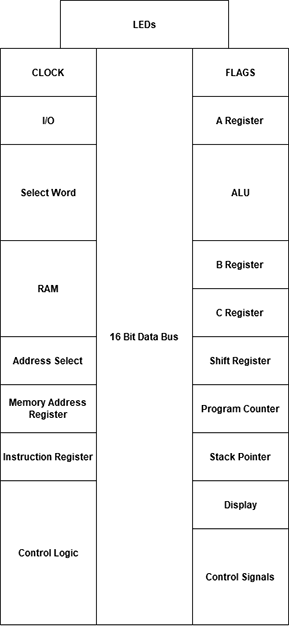
\includegraphics{16-bit-layout}
  \caption{High Level Module Overview and Layout of the 16-bit Breadboard Computer}
  \label{16-bit-layout}
\end{figure}
\clearpage

The updated computer specification contains the following modules, each of which will be followingly discussed in later sections:
\begin{enumerate}
  \item Common Data Bus \ref{common-data-bus}
  \item Data Bus LEDs \ref{data-bus-leds}
  \item Clock \ref{clock}
  \item A Register \ref{a-reg}
  \item B Register \ref{b-reg}
  \item Arithmetic-Logic Unit (ALU) \ref{alu}
  \item Flags Register \ref{flags}
  \item C Register \ref{c-reg}
  \item Shift Register \ref{shift-reg}
  \item Random Access Memory (RAM) \ref{ram}
  \item Program Counter \ref{pc}
  \item Stack Pointer \ref{stack-pointer}
  \item Display \ref{display}
  \item I/O \ref{io}
  \item Memory Address Register \ref{mar}
  \item Instruction Register \ref{ir}
  \item Word Selector \ref{word-select}
  \item Address Selector \ref{addr-select}
  \item Control Logic \ref{control-logic}
  \item Control Signals \ref{control-sigs}
  \label{module-list}
\end{enumerate}

\subsection{Common Data Bus} \label{common-data-bus}
The Common Data Bus acts as the communication medium of the computer. Drawing a parallel between \emph{computer design}
and \emph{human anatomy}, the data bus acts like the circulatory systems. It ensures all other components are connected
and can talk to each other. The Common Data Bus should be 16 bits wide, since the final system should have a word length of
16 bits. Since all other modules connect to the Data Bus, it makes sense to have it located centrally, between all other modules.
This way, no module has to have particularly long wires to interface with the Bus.

\subsection{Data Bus LEDs} \label{data-bus-leds}
This modules is as simple as it gets. It should be composed of just 16 LEDs, or Light Emitting Diodes, one on each Data Bus line,
so that whatever gets asserted at a certain point in time on the Bus can be visible. Besides this, it can also contain pull-down
resistors to ensure that, if no module asserts anything on the bus, it should default to low, or a logic 0.

\subsection{Clock} \label{clock}
The clock acts as the heart of the system. It provides a pulse under the form of a square wave, based on which all other components
do their job. The clock signal should be distributed to all other modules. Besides providing the square wave clock pulse an inverse,
or counter clock pulse should be available, as well as the ability to change the frequency and to completeley stop the square wave
and replace it with a manual button press for demonstrational and debugging purposes.
Finally, the clock should take in one signal as input, namely halt, or \emph{HLT},
which should completeley stop the clock regardless of operating mode. This will allow the computer to halt execution
if, for example, the program is finished. \\
\textbf{$Input Control Signals: HLT$} \\
\textbf{$Output Control Signals: CLK, \overline{CLK}$}

\subsection{A Register} \label{a-reg}
The A register is a 16-bit memory storage module. It should implement three functions. First, when its \emph{AI}
(A Register In) signal goes high, it should latch in the contents of the data bus on the rising edge of the next clock pulse.
The second function is to output its contents to the bus when its \emph{$\overline{AO}$} (A Register Out) signal goes low. Finally,
if the \emph{$\overline{RST}$} (Reset) signal goes low, it should clear out its contents and latch in a 0 on all bits. Additionally,
the A register should have a direct 16-bit connection to the \emph{Arithmetic Logic Unit}, or ALU \ref{alu}. \\
\textbf{$Input Control Signals: CLK, AI, \overline{AO}, \overline{RST}$}
\textbf{$Direct Connection to: ALU$}

\subsection{B Register} \label{b-reg}
Similarly to the A Register, the B Register should store 16 bits of data from the bus. It should have similar control signals,
\emph{BI, BO} and \emph{RST}, which perform equivalent functions. It should also have a direct 16-bit connection to the \emph{ALU}
\ref{alu}.
\textbf{$Input Control Signals: CLK, BI, \overline{BO}, \overline{RST}$}
\textbf{$Direct Connection to: ALU$}

\subsection{Arithmetic Logic Unit} \label{ALU}
The Arithemtic Logic Unit, or ALU, is the module responsible with data procesing. It takes the contents from\emph{both A and B
registers} \ref{a-reg} \ref{b-reg} directly and adds them up. Is the \emph{SU} (Subtract) signal is provided, the contents of the
B Register \ref{b-reg} will be subtracted from the contents of the A register. If the \emph{$\overline{\varepsilon O}$} (Sum Out)
is taken low, the contents of the  ALU will be asserted on the data bus. The ALU also has a direct connection to the Flags Register
\ref{flags}. Over this connection, the ALU should provide three flags:
\begin{itemize}
  \item Parity Flag: whether the \emph{Least Significant Bit} is 0 or 1
  \item Zero Flag: wheter the content of the ALU is 0
  \item Carry Flag: wheter the result of the operation of the ALU is cannot be expressed within 16 bits
\end{itemize}
\textbf{$Input Control Signals: \varepsilon O, SU$}
\textbf{$Direct Connection to: A Register, B register, Flags Register$}

\subsection{Flags Register} \label{flags}
The Flags Register is essential towards ensuring the Turing completeness of the computer being built. Based on the state of the
flags, the computer can make branch decisions, which reflect the fact that Turing machines can make selective decisions based
on the symbol it has just read.
Essentially, the flags register serves the purpose to latch in the three flags provided by the ALU \ref{alu}: the Parity Flag, the
Zero Flag and the Carry Flag. When the \emph{FI} (Flags In) signal is taken high, on the next clock pulse it should latch in the
contents of those flags. Besides this, the Flags Register should clear its contetns when the \emph{$\overline{RST}$} (Reset) signal
is taken low. There is a direct connection between the Flags Register and the Control Logic module, as the flags play a role in
deciding what to do next. \\
\textbf{$Input Control Signals: CLK, FI$}
\textbf{$Direct Connection to: ALU$}

\subsection{C Register} \label{c-reg}
The C Register serves as a general purpose 16-bit register. It has signals similar to the other two registers, A \ref{a-reg} and
B \ref{b-reg}. When \emph{CI} (C Register In) goes high, on the next clock pulse the register should latch in the data word
asserted on the bus in its storage. IF \emph{$\overline{CO}$} (C Register Out) goes low, the register should assert its contents
on the data bus. IF \emph{$\overline{RST}$} (Reset) goes low, it should clear its contents and latch in onyl zeroes. There should
be no direct connection between the C register and any other registers. \\
\textbf{$Input Control Signals: CLK, CI, \overline{CO}, \overline{RST}$}

\subsection{Shift Register} \label{shift-reg}
The Shift Register is the other module of the 16-bit breadboard computer capable of conducting data processing tasks. First and
foremost, it should act as a normal register, so it should latch in the bus contents on the next clock pulse if the \emph{SI}
(Shift Register In) signal goes high, asserts its contents to the bus if \emph{$\overline{SO}$} goes low, and clears it contents
if \emph{$\overline{RST}$} goes low. Besides this, if \emph{SFL} (Shift Left) goes high, on the next clock pulse it should shift its
contents to the left by one bit and insert a 0 at the least significant bit of the data word. Similarly, if \emph{SFR}
(Shift Right) goes high, on the next clock pulse it should shift its contents one bit to the right and insert a 0 at the most
significand bit of the data word. \\
\textbf{$Input Control Signals: CLK, SI, \overline{SO}, SFL, SFR, \overline{RST}$}

\subsection{Random Access Memory (RAM)} \label{ram}
Random Access Memory, or RAM, is the equivalent of the tape on a Turing machine. It can be read from and written to, and it should
be large enough to accommodate algorithms, data and variables; all at the same time. Memory is organised in addresses. Each address
should store one 16-bit word of memory. A 10-bit address is deemed to be sufficent, so the computer should have a
\(2^10*16 = 16K\) memory space. The RAM module should also have a direct connection to the \emph{Address Selector}
\ref{addr-select} and to the the \emph{Word Selector} \ref{word-select}. The Address Selector serves a 10-bit address to the
memory, while the word selector serves a 16-bit data word to the RAM. If the \emph{RI} (RAM In) signal goes high, on the next clock
pulse the RAM Module should latch in the data word served by the word selector at the address provided by the address
selector. If the \emph{RO} signal goes low, the RAM module should assert the data word stored at the address provided by the
address selector on the data bus. Additionally, based on two control signals originating from toggle switches, \emph{PROG} and
\emph{ARDUINO}, the signal which governs the RAM writes can be changed. If \emph{PROG} is low, that means the computer is in run
mode, and the \emph{RI} signal controls writes. If \emph{PROG} is high, then the computer is in programming mode, and the
write signal is chosen based on the \emph{ARDUINO} signal. If \emph{ARDUINO} is low, then the writes are manually controlled
using a simple push button. If it is high, then an external \emph{Arduino Mega} \cite{arduino2020mega} controls the writes to
memory using a signal called \emph{$ARDUINO_WRITE$}. \\
\textbf{$Input Control Signals: CLK, RI, RO, PROG, ARDUINO, ARDUINO_WRITE$} \\
\textbf{$Direct Connection to: Word Selector, Address Selector, Arduino Mega$}

\subsection{Program Counter} \label{pc}
The Program Counter serves the purpose of keeping track of the current address which should be executed. As such, it should
be a 10-bit register, to ensure coverage of the entire address space of the computer. If the \emph{CE} (Counter Enable) signal
goes high, on the next clock cycle the program counter should count up one in binary from the value it has currently latched
in its storage and then latch this new value in. If the \emph{$\overline{JMP}$} (Jump) signal goes low, on the next clock pulse the
program counter should latch in whatever value is asserted on the 10 loweest bits of the bus in its register. If
\emph{$\overline{CNT_O}$} (Counter Out) goes low, the value latched in the program counte should be asserted on the data bus.
If \emph{$\overline{RST}$} (Reset) goes low, the program counter should clear out its contents and latch in zeroes on all bits. \\
\textbf{$Input Control Signals: CLK, CE, \overline{JMP}, \overline{CNT_O}, \overline{RST}$}

\subsection{Stack Pointer} \label{stack-pointer}
Tha stack pointer should essentially be a register holding a 10-bit address, but accepting only a small subsection of the address
space (from 0x3F0 to 0x3F). This means that the stack should be 16 addresses tall. If the \emph{$\overline{ST_I}$} (Stack Increment)
signal goes low, on the next clock pulse, the stack pointer should increment by one. If \emph{$\overline{ST_D}$} (Stack Decrement)
goes low, the stack pointer should decrement by one on the next clock pulse.
On \emph{$\overline{ST_J}$} (Stack Jump) going low, on the next clock pulse the stack pointer should latch in the address asserted
on the bus in its register, assuming it is a valid stack address. If \emph{$\overline{ST_O}$} goes low, the stack pointer should
assert the address it has stored out on the bus. Finally, if \emph{$\overline{RST}$} (Reset) goes low, the stak pointer should reset
to zero. \\
\textbf{$Input Control Signals: CLK, \overline{ST_I}, \overline{ST_D}, \overline{ST_J}, \overline{ST_O}, \overline{RST}$}

\subsection{Display} \label{display}
The Display module is the main way through which the computer can interface with the user. It should have the ability to display
both alfanumeric characters and digits and it should feature at least 2 lines of 16 characters each. When the \emph{OUT} (Output)
signal goes high, the display should take a word of data from the bus and interpret it as the next character to be written to the
screen. \\
\textbf{$Input Control Signals: OUT$}

\subsection{I/O} \label{io}
Besides a display, the computer should also feature a bidirectional interface to another mirocontroller. In this case,
the interface should be to an \emph{Arduino Mega} \cite{arduino2020mega}. If the \emph{$\overline{E}$} (Enable) signal goes low,
based on the \emph{$R/\overline{W}$} (Read/Write) signal, the computer should interact with the Arduino. If the
\emph{$R/\overline{W}$} signal is high the computer should read a word of data from the arduino, so that word of data should be
asserted on the bus. If the \emph{$R/\overline{W}$} signal is low, the Arduino should read a word of data from the bus (and
consequently displayed to the user). \\
\textbf{$Input Control Signals: \overline{E}, R/\overline{W}$} \\
\textbf{$Direct Connection to: Arduino Mega$}

\subsection{Memory Address Register} \label{mar}
The memory address register, or MAR, is a 10 bit register. It connects directly to the address selector \ref{address-select} and
there is no other way to get the information latched into it. If the \emph{MI} signal goes high, on the next clock pulse the MAR
will latch into its storage the 10 least significant bits asserted on the bus. if \emph{$\overline{RST}$} goes low, the MAR will
clear its contents and write zeroas to all 10 bits. \\
\textbf{$Input Control Signals: CLK, MI, \overline{RST}$} \\
\textbf{$Direct Connection to: Address Selector$}


\subsection{Instruction Register} \label{ir}
The Instruction Register, or IR, is a 16-bit register which holds the next instruction to be processed. It is special in that
its most significant 6 bits have a different meaning. They represent the opcode for the current instruction and are directly
connected to the Control Logic module \ref{control-logic}. When the \emph{II} (Instruction Register In) signal goes high, on the
next clock pulse the instruction register should latch in the data word asserted on the bus in its storage. If the
\emph{$\overline{IO}$} (Instruction Register Out) signal goes low, the register should assert its least significand 10 bits to the
bus. If \emph{$\overline{RST}$} (Reset) goes low, the instruction register should reset and latch in zeroes on all 16 bits. \\
\textbf{$Input Control Signals: CLK, II, \overline{IO}$} \\
\textbf{$Direct Connection to: Control Logic$}


\subsection{Word Selector} \label{word-select}
The Word Selector is a special module, in that it serves the purpose of selecting between different sources of data and feeding
them into the RAM module \ref{ram}. There are three possible sources of data
\begin{enumerate}
  \item The Data Bus
  \item Dip Switches
  \item An Arduino Mega
\end{enumerate}
The Data Bus is the first and most straight forward data source. A 16-bit data word can be taken from the bus and then passed on
to memory. The second source are Dip Switches. Dip Switches are rows of small binary switches, which can be used to manually feed
binary data into a digital system. The last possible source of data is an arduino mega. The choice of data to be fed forward is
governed by two control signals, \emph{PROG} and \emph{ARDUINO}. If \emph{PROG} is low, data from the data bus will be selected,
regardless of the state of \emph{ARDUINO}. If \emph{PROG} is high, that means that the computer is in programming mode. In this
mode, the data source depends on the \emph{ARDUINO} control signal. If this signal is high, then data will be fed forward from
an external Arduino Mega \cite{arduino2020mega}. If it is low, then a series of 16 dip switches will be used to manually program
the computer.  \\
\textbf{$Input Control Signals: PROG, ARDUINO$} \\
\textbf{$Direct Connection to: RAM, Arduino Mega$}

\subsection{Address Selector} \label{address-select}
Similar to the Word Selector \ref{word-select}, the Address Selector selects between different address sources to provide a 10-bit
address to  the RAM module \ref{ram}. There are three possible data sources:
\begin{enumerate}
  \item The Memory Address Register \ref{mar}
  \item Dip Switches
  \item An Arduino Mega
\end{enumerate}
The choice of data source is defined by two control signals, \emph{PROG} and \emph{ARDUINO}. If \emph{PROG} is low, then the
computer is in run mode and the address latched in the \emph{MAR} \ref{mar} is fed forward to RAM. If it is high, then that means
the computer is in programming mode and the address choice is governed by the \emph{ARDUINO} control signal. If it is low, then
the memory address will be manually chosen using a series of 10 Dip Switches. If it is high, then an external
Arduino Mega \ref{arduino2020mega} will be the address source. \\
\textbf{$Input Control Signals: PROG, ARDUINO$}
\textbf{$Direct Connection to: RAM, Arduino Mega$}

\subsection{Control Logic} \label{control-logic}
To draw another parallel to human anatomy, the control logic module can be thought of as the ~~brain`` of the computer.
It takes in the 6-bit opcode from the Instruction Register \ref{ir}, the 3 flags from the Flags Register \ref{flags}, as well as
a 3 bit number representing the ~~step`` of the current instruction which is to be executed and decides based on these pieces
of information which control signals to keep active on the next clock cycle. It also maintains an internal 3 bit counter which
counts on the inverted clock or counter clock signal to provide the 3-bit step. \\
\textbf{$Input Control Signals: \overline{CLK}$}
\textbf{$Output Control Signals: HLT, \overline{RST}, AI, \overline{AO}, BI, \overline{BO}, \overline{\varepsilon O}, SU, FI, CI, \overline{CO}, SI, \overline{SO}, SFL, SFR, RI, RO, CE, \overline{JMP}, \overline{CNT_O}, \overline{ST_I}, \overline{ST_D}, \overline{ST_J}, \overline{ST_O}, OUT, \overline{E}, R/\overline{W}, MI, II, \overline{IO}$}
\textbf{$Direct connection to: Instruction Register, Flags Register$}


\subsection{Control Signals} \label{control-sigs}
The Control Signals Module is used to visualise which control signals are active at any given time. This module should
essentially consist of a labeled LED on each control signal.

\section{Specification Conclusion}
This concludes the specification phase of the project. The next step is to design each module to this specification.
